 \subsubsection{UC8 - Gestione Veicoli}
  \begin{figure}[H]
 	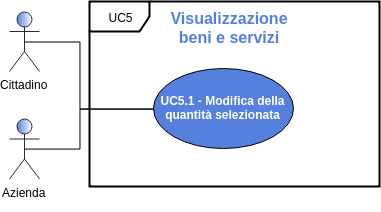
\includegraphics[width=6cm]{res/images/UC5-Generale.png}
 	\centering
 	\caption{UC5 - Gestione Veicoli}
 \end{figure}
 \begin{itemize}
 	\item \textbf{Attori Primari}: utente autenticato;
 	\item \textbf{Descrizione}: l'utente visualizza i propri veicoli. Per ogni veicolo vengono visualizzate le seguenti informazioni:
 	\begin{itemize}
 		\item marca;
 		\item modello;
 		\item rating;
 	\end{itemize}
 	\item \textbf{Precondizione}: l'utente accede al fragment\glosp per la gestione dei veicoli;
 	\item \textbf{Postcondizione}: l'utente visualizza le informazioni relative ai propri veicoli, con le eventuali operazioni disponibili su ognuno di essi.
 \end{itemize}
 \subsubsection{UC5.1 - Aggiunta Veicolo}
 \begin{itemize}
 	\item \textbf{Attori Primari}: utente autenticato;
 	\item \textbf{Descrizione}: l'utente può aggiungere un mezzo di trasporto al proprio parco macchine;
 	\item \textbf{Scenario principale}: l'utente aggiunge un veicolo; l'utente attraverso appositi campi ne deve specificare marca e modello;
 	\item \textbf{Precondizione}: l'utente sta visualizzando un prodotto ed intende modificarne la quantità selezionata;
 	\item \textbf{Postcondizione}: la quantità del prodotto è stata aggiornata al nuovo valore selezionato.
 \end{itemize}